\documentclass[a4paper,12pt]{article} 

%%% Работа с русским языком
\usepackage{cmap}					% поиск в PDF
\usepackage{mathtext} 				% русские буквы в фомулах
\usepackage[T2A]{fontenc}			% кодировка
\usepackage[utf8]{inputenc}			% кодировка исходного текста
\usepackage[english,russian]{babel}	% локализация и переносы

%%% Дополнительная работа с математикой
\usepackage{amsmath,amsfonts,amssymb,amsthm,mathtools, gensymb} % AMS
\usepackage{icomma} % "Умная" запятая: $0,2$ --- число, $0, 2$ --- перечисление

%%Таблица
\usepackage[table,xcdraw]{xcolor}
\usepackage{caption}
\usepackage{subcaption}
\usepackage{floatrow}
\floatsetup[table]{capposition=top}
\floatsetup[wrapfigure]{capposition=bottom}
%multi-column
%\usepackage{multi-column}
%multi-row
\usepackage{multirow}


%% Номера формул
\mathtoolsset{showonlyrefs=true} % Показывать номера только у тех формул, на которые есть \eqref{} в тексте.

%% Шрифты
\usepackage{euscript}	 % Шрифт Евклид
\usepackage{mathrsfs} % Красивый матшрифт

%% Свои команды
\DeclareMathOperator{\sgn}{\mathop{sgn}}

%% Перенос знаков в формулах (по Львовскому)
\newcommand*{\hm}[1]{#1\nobreak\discretionary{}
{\hbox{$\mathsurround=0pt #1$}}{}}

%% Стиль страницы
\usepackage{fancyhdr}

%% Для рисунков
\usepackage{graphicx}
\usepackage[export]{adjustbox}
\usepackage{float}
\usepackage{ragged2e}
\usepackage{wrapfig}

%Отступы и поля 
\textwidth=20cm
\oddsidemargin=-2cm
\topmargin=-2cm
\textheight=25cm

\pagestyle{fancy}
\begin{document}
\begin{titlepage}
\begin{center}
%\vspace*{1cm}
\large{\small ФЕДЕРАЛЬНОЕ ГОСУДАРСТВЕННОЕ АВТОНОМНОЕ ОБРАЗОВАТЕЛЬНОЕ\\ УЧРЕЖДЕНИЕ ВЫСШЕГО ОБРАЗОВАНИЯ \\ МОСКОВСКИЙ ФИЗИКО-ТЕХНИЧЕСКИЙ ИНСТИТУТ\\ (НАЦИОНАЛЬНЫЙ ИССЛЕДОВАТЕЛЬСКИЙ УНИВЕРСИТЕТ)\\ ФАКУЛЬТЕТ АЭРОКОСМИЧЕСКИХ ТЕХНОЛОГИЙ}
\vfill
\line(1,0){430}\\[1mm]
%\huge{Лабораторная 2}\\
\huge\textbf{Изгиб балки}\\
\line(1,0){430}\\[1mm]
\vfill
\begin{flushright}
\normalsize{Рогозин Владимир}\\
\normalsize{\textbf{Группа Б03-106}}\\
\end{flushright}
\end{center}
\end{titlepage}
\fancyhead[c] {Изгиб балки}

\textbf{Цель работы:} 
1) Ознакомление с теорией изгиба статически определимых и статически неопределимых балок, в частности, с теорией Костилиано.\\
2) Экспериментальное подтверждение методов расчёта статически неопределимых балок.

\textbf{Теоретические сведения:} 
Рассмотрим изгиб однородного бруса (балки) произвольного постоянного поперечного сечения на рис. 1. Ввиду бесконечной малости выделенного элемента можно считать, что в результате изгиба прямые $АА', NN', ВВ'$ и все прямые, им параллельные, перейдут в окружности с центрами, лежащими на оси О, перпендикулярной к плоскости рисунка.

\begin{figure}[H]\label{fig:izgib_Sivukhin} 
    \centering
    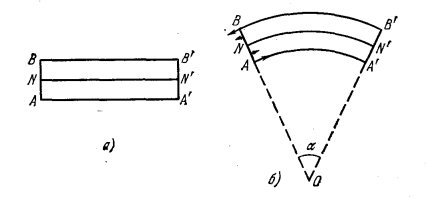
\includegraphics[width = \textwidth]{Izgib.png}
    \caption{а) Балка в покоящемся состоянии, б) изогнутая балка}
\end{figure}
 Эта ось называется осью изгиба. Наружные волокна, лежащие выше
линии $NN'$, при изгибе удлиняются, волокна, лежащие ниже линии $NN
'$, — укорачиваются. Длина линии $NN'$ остается неизменной. Эта линия называется \textit{нейтральной} линией. Проходящее через нее сечение (недеформированного) бруса плоскостью, перпендикулярной к плоскости рисунка называется \textit{нейтральным} сечением. Пусть $R$ — радиус кривизны нейтральной линии. Рассмотрим удлинение волокна бруса, находящегося на расстоянии $\xi$ от нейтральной линни.  Если брус не слишком толст, так что $|\xi| \ll R$, то длина рассматриваемого волокна будет $l = (R + \xi) \alpha$, а удлинение $\Delta l = l - l_0 = \xi \alpha$. Получаем натяжение вдоль рассматриваемого волокна 
\[\tau = E \frac{\xi}{R},\]
отсюда момент сил, действующий на брусок относительно оси, перпендикулярной рисунку и проходящей через середину нейтральной линии
\[M_\tau = \frac{E}{R}\int \xi^2 dS = \frac{EJ}{R},\]
где обозначен осевой момент инерции
\[J = \int \xi^2 dS.\]
Вспоминая выражение для радиуса кривизны
\[\frac{1}{R} = \frac{y''}{(1 + (y')^2)^{3 / 2}}.\]
при малых изгибах можно пренебречь квадратом производной. Окончательно запишем выражение для момента сил, действующих внутри стержня
\[M_\tau = EJy''.\]

При нагрузке балки в её сечении возникает \textit{изгибающий момент}. Запишем уравнения равновесия для балки
\[
    \left\{
    \begin{aligned}
        &R_A + R_B - P = 0, \\
        &R_B \cdot 2a + M_A - P \cdot a = 0. 
    \end{aligned}
    \right
\]

\begin{figure}[H]\label{fig:izgib} 
    \centering
    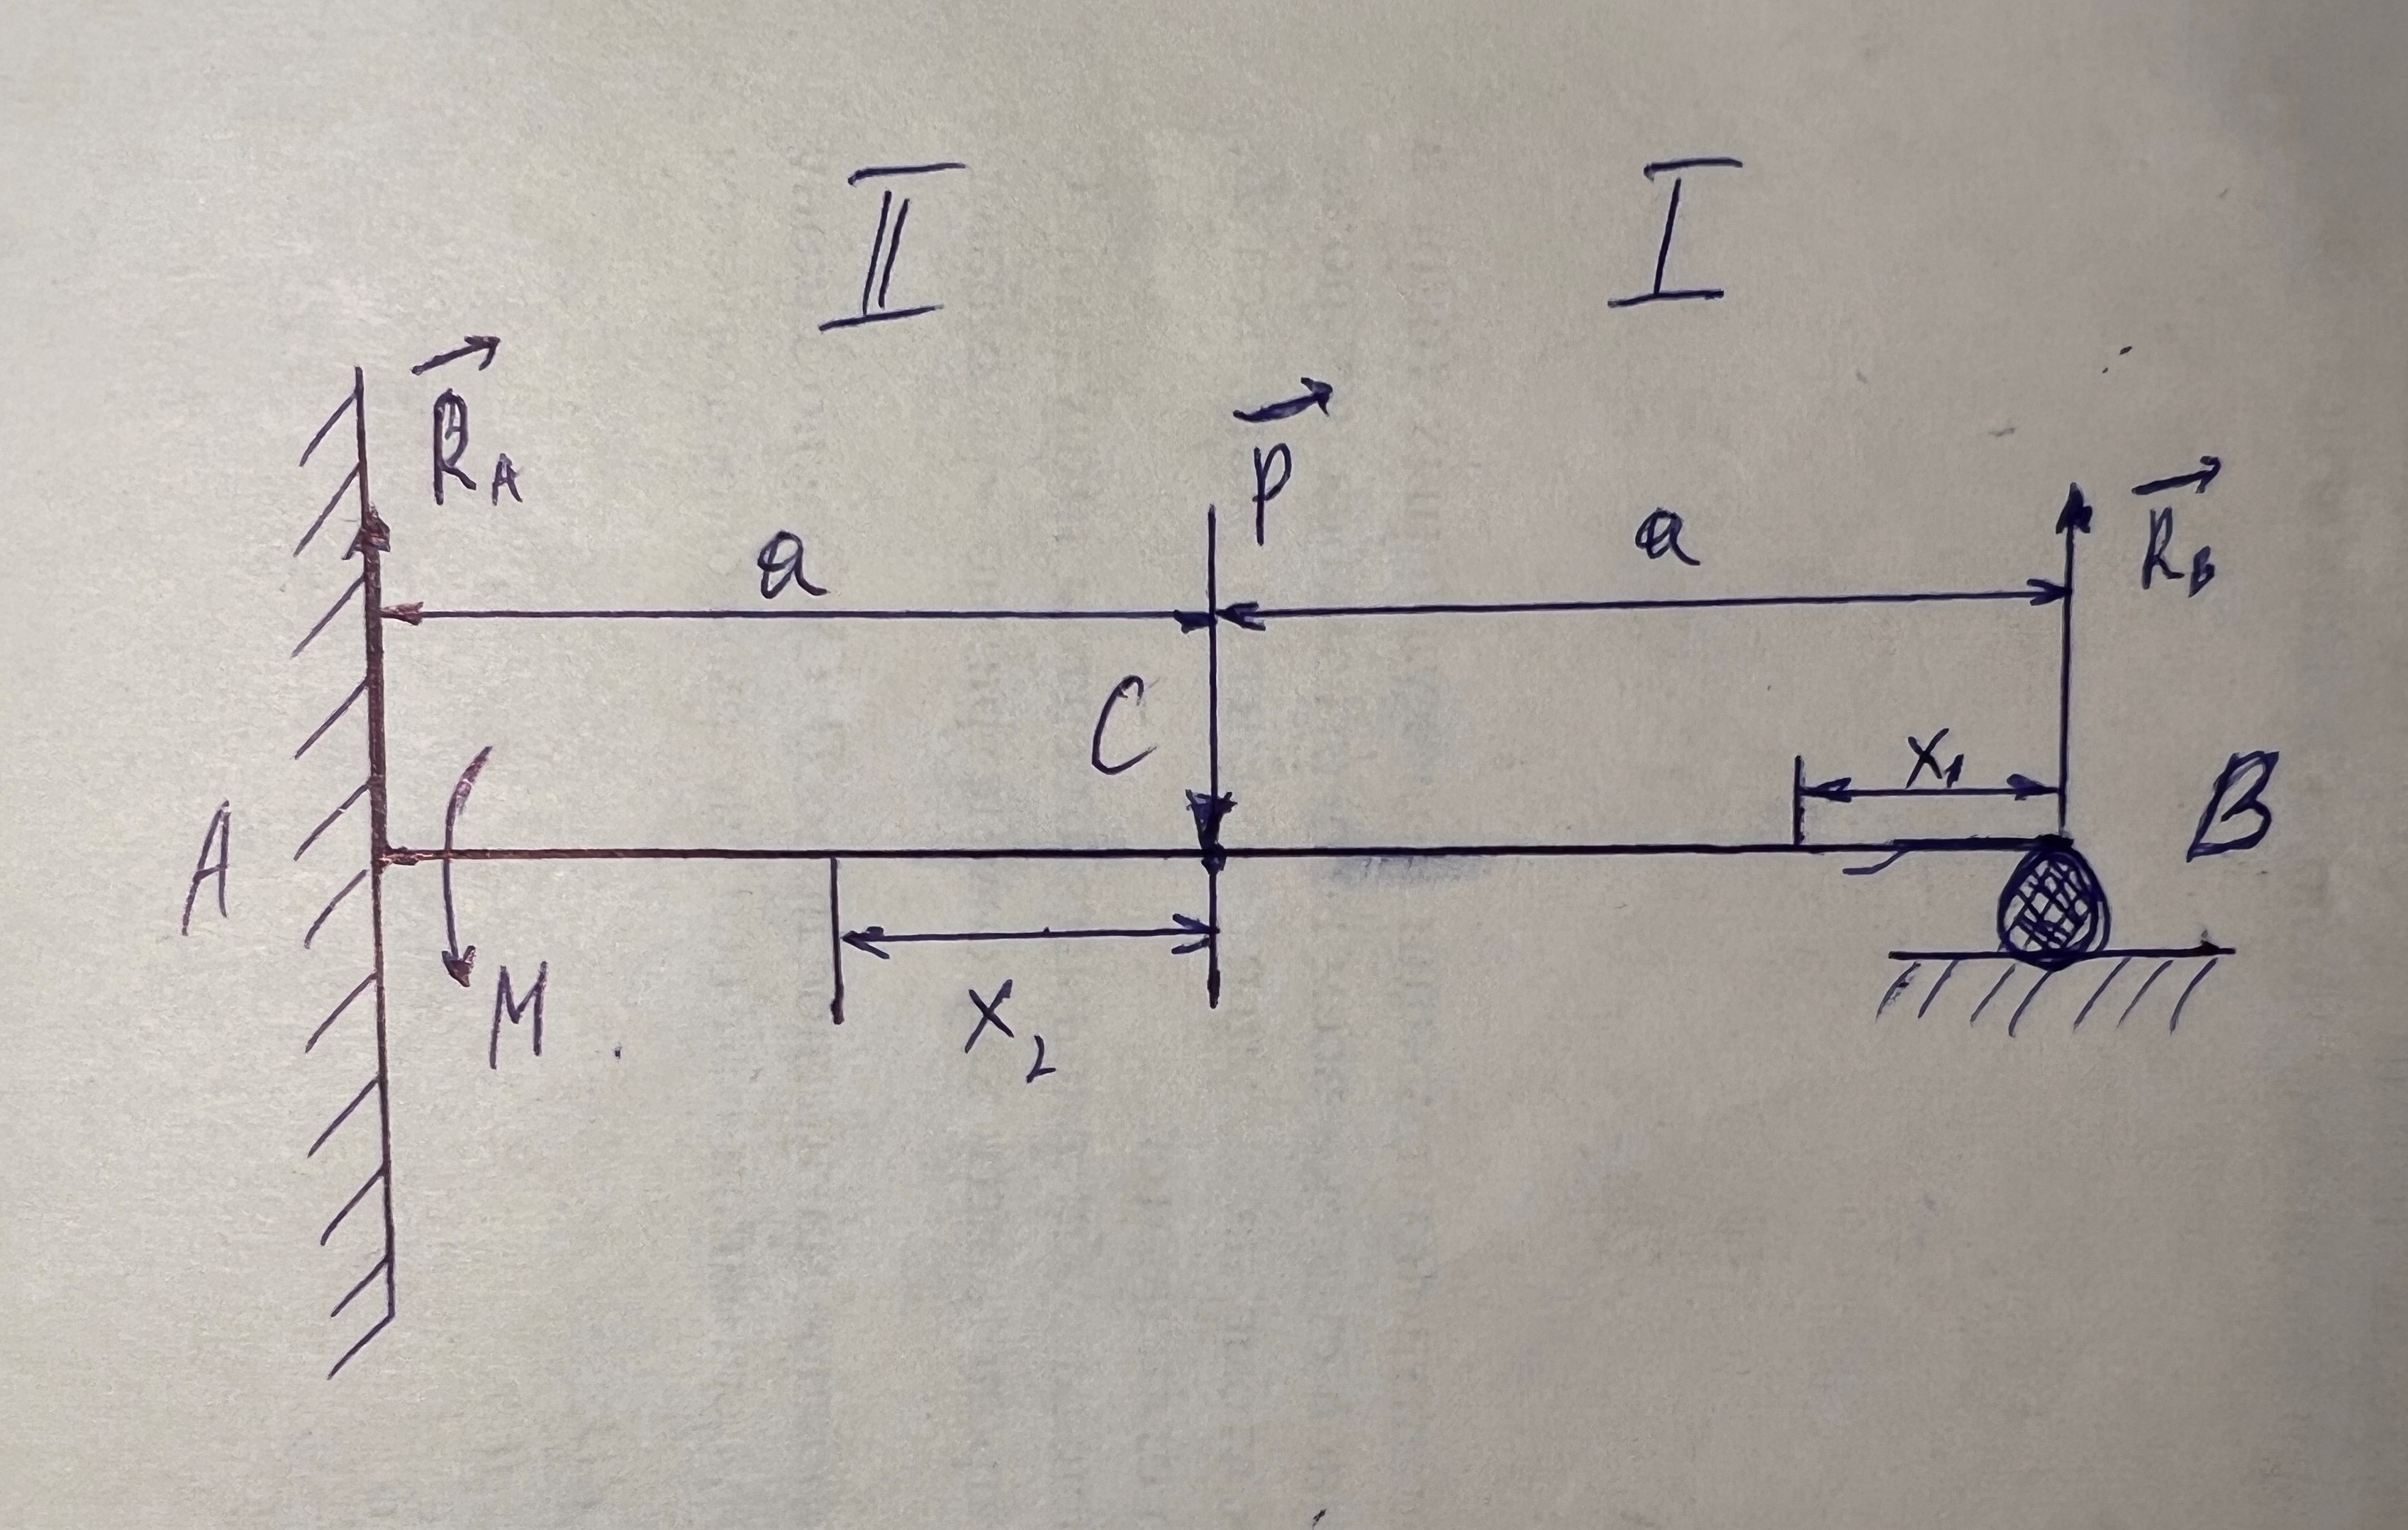
\includegraphics[width = 0.8\textwidth]{Изгиб.jpg}
    \caption{Статически неопределимая балка}
\end{figure}

Задача один раз статически неопределима. Для получения дополнительного соотношения воспользуемся \textit{теоремой Кастилиано}, которая записывается в виде
\[y_i = \frac{\partial W}{\partial P_i},\]
где $W$ -- полная упругая энергия системы, $P_i$ -- $i$-я приложенная точечная сила, $y_i$ -- перемещению точки приложения силы $P_i$ в направление её действия.

При изгибе балки упругую энергию системы можно записать в виде 
\[W = \int M d\alpha = \int \frac{1}{2} M(x) d\alpha = \int \frac{1}{2} M(x) \frac{dx}{R} = \int \frac{1}{2} \frac{M(x)^2}{E J} dx,\]
где $M(x)$ -- изгибающий момент, $E$ -- модуль Юнга материала, $J$ -- осевой момент инерции. Тогда для смещения приложения силы получаем выражение
\begin{equation}\label{eq: y_i via M}
    y_i = \frac{1}{E J} \int M(x) \frac{\partial M(x)}{\partial P_i} dx.
\end{equation}

Так как в точке $B$ смещение равно нулю, то можем записать недостающее уравнение для нашей системы
\[y_B = 0 = \frac{1}{E J} \int M(x) \frac{\partial M(x)}{\partial R_B} dx.\]

Распишем момент, действующий в балке, на два слагаемых 
\begin{equation}\label{eq: M_1 and M_2}
    M_I(x) = R_B \cdot x_1, \quad M_{II}(x) = R_B \cdot (x_2 + a) - P \cdot x_2;
\end{equation}
\begin{equation}\label{eq: M_1' and M_2'}
    \frac{\partial M_I(x)}{\partial R_B} = x_1, \quad \frac{\partial M_{II}(x)}{\partial R_B} = a + x_2;
\end{equation}

\[0 = \int\limits_0^a R_B x_1^2 dx_1 + \int\limits_0^a (R_B (a + x_2) - P x_2)(a + x_2) dx_2.\]

Интегрируя, получаем дополнительное соотношение 
\begin{equation}\label{eq: R_B(P)}
    R_B = \frac{5}{16} P.
\end{equation}

Нагрузим балку силой $P = 5 кг$, рассчитаем теоретическое значение $R_B$ и сравним его с экспериментальным. Результаты представлены в таблице ниже.  
\begin{table}[H]\label{tab: Result R_B}
    \centering
    \begin{tabular}{|
        >{\columncolor[HTML]{FFFFFF}}c |
        >{\columncolor[HTML]{FFFFFF}}c |
        >{\columncolor[HTML]{FFFFFF}}c |
        >{\columncolor[HTML]{FFFFFF}}c |}
        \hline
        {\color[HTML]{000000} }         & {\color[HTML]{000000} Теория} & {\color[HTML]{000000} Эксперимент} & {\color[HTML]{000000} $\varepsilon$, \%} \\ \hline
        {\color[HTML]{000000} $R_B$, Н} & {\color[HTML]{000000} 15,3} & {\color[HTML]{000000}16,9}           & {\color[HTML]{000000} 10,5}                  \\ \hline
    \end{tabular}
    \caption{Результаты для силы реакции $R_B$}
\end{table}

Далее, используя ранее полученные соотношения, вычислим $y_C$ -- прогиб балки в точке $C$, потом измерим значение прогиба в этой точке и сравним с вычисленным теоретически. Для этого подставим \eqref{eq: R_B(P)} в \eqref{eq: M_1 and M_2} и воспользуемся выражением \eqref{eq: y_i via M}. Параметры системы представлены в таблице ниже.

\begin{table}[H]\label{tab: Params of system}
    \centering
    \begin{tabular}{|
        >{\columncolor[HTML]{FFFFFF}}c |
        >{\columncolor[HTML]{FFFFFF}}c |
        >{\columncolor[HTML]{FFFFFF}}c |
        >{\columncolor[HTML]{FFFFFF}}c |}
        \hline
        {\color[HTML]{000000} $E$, $кг / см^2$} &
          {\color[HTML]{000000} $h$, мм} &
          {\color[HTML]{000000} $b$, мм} &
          {\color[HTML]{000000} $a$, cм} \\ \hline
        {\color[HTML]{000000} $2 \cdot 10^6$} &
          {\color[HTML]{000000} 24,1} &
          \cellcolor[HTML]{FFFFFF}{\color[HTML]{000000} 6,2} &
          \cellcolor[HTML]{FFFFFF}{\color[HTML]{000000} 33,3} \\ \hline
    \end{tabular}
    \caption{Параметры системы}
\end{table}

Осевой момент инерции выражается через $b$ и $h$ как 
\[J = \frac{h b^3}{12}\]

Тогда для прогиба балки в точке $C$ получим выражение
\[y_C = \frac{12}{E h b^3}\bigg[ \int\limits_0^a \frac{25}{16^2} P \cdot x_1^2 dx_1 +  \int\limits_0^a \frac{P}{16^2} (5a - 11x_2)^2 dx_2 \bigg]\]
\[y_C = \frac{12}{E h b^3} \bigg(\frac{25}{768} P a^3 + \frac{31}{768} P a^3\bigg) = \frac{7}{8} \frac{P a^3}{E h b^3}\]

\begin{table}[H]\label{tab: Result y_C}
    \centering
    \begin{tabular}{|
        >{\columncolor[HTML]{FFFFFF}}c 
        >{\columncolor[HTML]{FFFFFF}}c 
        >{\columncolor[HTML]{FFFFFF}}c 
        >{\columncolor[HTML]{FFFFFF}}c |}
        \hline
        \multicolumn{4}{|c|}{\cellcolor[HTML]{FFFFFF}{\color[HTML]{000000} $P = 51,5$ H}} \\ \hline
        \multicolumn{1}{|c|}{\cellcolor[HTML]{FFFFFF}{\color[HTML]{000000} }} &
          \multicolumn{1}{c|}{\cellcolor[HTML]{FFFFFF}{\color[HTML]{000000} Теория}} &
          \multicolumn{1}{c|}{\cellcolor[HTML]{FFFFFF}{\color[HTML]{000000} Эксперимент}} &
          {\color[HTML]{000000} $\varepsilon,$ \%} \\ \hline
        \multicolumn{1}{|c|}{\cellcolor[HTML]{FFFFFF}{\color[HTML]{000000} $y_C,$ мм}} &
          \multicolumn{1}{c|}{\cellcolor[HTML]{FFFFFF}{\color[HTML]{000000} 1,48}} &
          \multicolumn{1}{c|}{\cellcolor[HTML]{FFFFFF}{\color[HTML]{000000} 1,73}} &
          {\color[HTML]{000000} 16,9} \\ \hline
    \end{tabular}
    \caption{Результаты для прогиба $y_C$}
\end{table}

%\textbf{Обработка данных:}

%\textbf{Вывод:} 

\end{document}
